\documentclass[11pt,letterpaper]{article}
\usepackage[margin=0.82in,headheight=15pt]{geometry}
\usepackage[T1]{fontenc}
\usepackage{lmodern,amsmath,amssymb,mathtools,booktabs,array,graphicx}
\usepackage{xcolor,microtype,enumitem,fancyhdr}
\definecolor{navy}{HTML}{18384E}\definecolor{teal}{HTML}{137F8C}\definecolor{pale}{HTML}{EDF4F6}
\usepackage[colorlinks=true,linkcolor=navy,urlcolor=teal,citecolor=navy]{hyperref}
\hypersetup{pdftitle={Radion kinetics and scalar mixing in the exact spectral vacuum},pdfauthor={Prepared for Christopher Michael Baird with OpenAI Codex}}
\pagestyle{fancy}\fancyhf{}
\fancyhead[L]{\small\color{navy} MQGT--SCF / RADION AND SCALAR DYNAMICS}
\fancyhead[R]{\small 22 October 2026}
\fancyfoot[L]{\small Exact internal sums; two external derivatives}
\fancyfoot[R]{\small\thepage}
\setlength{\parindent}{0pt}\setlength{\parskip}{5pt}
\setlist{nosep,leftmargin=1.5em}\emergencystretch=2em
\widowpenalty=10000\clubpenalty=10000
\DeclareMathOperator{\Tr}{Tr}\DeclareMathOperator{\diag}{diag}
\newcommand{\dd}{\mathrm d}\newcommand{\Lam}{\Lambda}
\newcommand{\B}{\mathcal B}\newcommand{\HH}{\mathcal H}
\newcommand{\GE}{G^{\mathrm E}}\newcommand{\GJ}{G^{\mathrm J}}
\newcommand{\BranchTable}{\begin{tabular}{llrrrrrr}\toprule $\epsilon$ & Profile & $f$ & $G^E_{RR}$ & $m_C^2$ & $m_1^2$ & $m_2^2$ & $m_r^2$\\\midrule
$0.01$ & $f_{-}$ & 0.211384912 & 0.356376269 & 0.0081547747 & 0.0099066681 & 0.020157812 & 0.8295963 \\
$0.01$ & $f_{+}$ & 0.211384910 & 0.356375864 & 0.0081547437 & 0.0099066304 & 0.020157731 & 0.82958471 \\
$0.0001$ & $f_{-}$ & 0.212137457 & 0.356410811 & 8.1088724e-05 & 9.8398e-05 & 0.00020001574 & 0.83274432 \\
$0.0001$ & $f_{+}$ & 0.212137459 & 0.356410386 & 8.1060978e-05 & 9.836433e-05 & 0.00019994727 & 0.83273277 \\\bottomrule\end{tabular}}
\newcommand{\JordanMatrix}{\begin{pmatrix}-0.3059242 & 0.0048923 & 0.0034082\\0.0048923 & 0.0581066 & -0.0001103\\0.0034082 & -0.0001103 & 0.0436358\end{pmatrix}}
\newcommand{\EinsteinMatrix}{\begin{pmatrix}0.3563763 & -0.0034422 & -0.0024035\\-0.0034422 & 0.0582115 & -0.0000371\\-0.0024035 & -0.0000371 & 0.0436868\end{pmatrix}}
\newcommand{\PhaseMatrix}{\begin{pmatrix}0.0584073 & -0.0000555\\-0.0000555 & 0.0438309\end{pmatrix}}
\newcommand{\ChargedMatrix}{\begin{pmatrix}0.0584545 & -0.0000774\\-0.0000774 & 0.0437877\end{pmatrix}}

\begin{document}
\thispagestyle{plain}
{\small\bfseries\color{teal} BAIRD / ZORAASI RESEARCH CONTINUATION}\par
{\LARGE\bfseries\color{navy} Radion kinetics and scalar mixing\\ in the exact spectral vacuum}\par
{\large Two-derivative dynamical tests and the near-cutoff radion limitation}\par
\textbf{Prepared for Christopher Michael Baird with OpenAI Codex}\hfill 22 October 2026

\colorbox{pale}{\parbox{\dimexpr\linewidth-2\fboxsep\relax}{\textbf{Result.} The declared warped-product Dirac operator determines the radion kinetic term, its scalar mixing, and the field-dependent gravitational coefficient by convergent internal spectral representations. The Jordan-frame radion coefficient is negative at the tuned fixtures, but its Einstein-frame completion is positive. The full nine-dimensional radius/lowest-scalar kinetic matrix is positive for both profiles at both tunings. The two-derivative mass problem has five positive parameters and four gauge zeros; a positive, potential-free axion sector leaves one additional physical massless phase after gauge reduction. The radion-dominated parameter is near $0.91\Lam$, beyond a demonstrated low-momentum hierarchy. These are restricted infrared stability tests, not full propagator, ultraviolet, or compactification stability results.}}

\section{Question, preserved inputs, and scope}

The exact coupled-vacuum note \cite{vacuum} found a runaway in the untuned action and constructed restricted stationary branches after an explicitly selected scalar-mass counterterm and a separately selected flatness subtraction. Its static Hessian was positive transverse to symmetry zeros, but the radion kinetic term and its mixing with the scalars were missing. This note supplies those coefficients from the same operator and tests the resulting two-external-derivative action.

The source is pinned at commit \texttt{8ac07febf9b760720b9c5e85898499c7195e2dde}. The inherited \texttt{mode\_sums.py}, \texttt{vacuum.py}, common-vacuum input and numerical branch records are copied unchanged; their hashes are in \texttt{provenance.json}. We retain four copied fermion blocks, unit dimensionless Yukawas, a fixed equivariant monopole connection, and the two lowest scalar harmonics on a round sphere. The tuned parameters are $\epsilon=10^{-2},10^{-4}$, with the same mass counterterm $\alpha$ for the two profiles and separately chosen $c$.

Here exactness refers to the internal representation and all powers of retained scalar amplitudes. The numerical sums use finite angular cutoffs. The external spacetime dependence is retained only through two derivatives, apart from a clearly identified fixed-metric momentum diagnostic. No finite local expansion in $1/R$ replaces the internal sums. The spectral function is denoted $f_{\rm sp}$ below; the separate symbol $f=F/(\kappa\Lam^2)$ denotes the gravitational coefficient.

\section{Warped operator and a common spinor Hilbert space}

Promote the radius to a spacetime field in the torsion-free metric
\begin{equation}
 \dd s_6^2=g_{\mu\nu}(x)\dd x^\mu\dd x^\nu+r(x)^2\dd\Omega_2^2,
 \qquad R=\Lam r,\quad h_i=H_i/(\Lam R),\quad\kappa>0.
 \label{eq:metric}
\end{equation}
The monopole connection and angular basis are held fixed under this identification. With Euclidean Hermitian gamma matrices, the warped Dirac operator is
\begin{equation}
 D_{6,\Phi}=D_g+i\gamma^\mu\partial_\mu\ln r
       +\gamma_5\Lam\B(R,h),\qquad
 \B=D_{\rm int}/R+\sum_i h_i S_i .
 \label{eq:warpedD}
\end{equation}
The coefficient of $\partial\ln r$ is half the fibre dimension, hence one. This follows from the warped spin connection; it also specializes the even-base formula of \cite{warped}. The charged monopole connection adds the inherited fibre operator and does not change that coefficient. Complex scalar tangents are included as Hermitian real-coordinate variations of $\B$.

The unitary map from the measure $\sqrt g\,r^2\dd^4x\dd\Omega$ to $\sqrt g\dd^4x\dd\Omega$ is $\chi=r\psi$. Consequently
\begin{equation}
 rD_{6,\Phi}r^{-1}=D_g+\gamma_5\Lam\B(R,h).
 \label{eq:unitary}
\end{equation}
The derivative of $r^{-1}$ cancels the connection term in \eqref{eq:warpedD}. This is an equivalence of classical spectral traces, not a quantum path-integral change of measure. Adding a second independent ``radion kinetic term'' after evaluating \eqref{eq:unitary} would double count the same geometry. Conversely, differentiating the constant-radius eigenvalues without including their scalar-dependent eigenvectors would miss transition matrix elements.

For the neutral background the three sectors are
\begin{equation}
 B_q=D_{2\oplus1\oplus1}/R+h_dS_d+h_uS_u,\quad
 B_\ell=D_{2\oplus1}/R+h_dS_\ell,\quad B_0=D_0/R.
\end{equation}
Their full internal trace multiplicities are $n_q=12$, $n_\ell=4$, $n_0=12$. These include colour and four copies, while the action retains its original factor $\kappa/2$:
\begin{equation}
 S_{\rm sp}=\frac\kappa2\Tr_{\rm Dirac} f_{\rm sp}(D_{6,\Phi}^2/\Lam^2),
 \quad f_{\rm sp}(z)=\sum_a w_ae^{-az},\quad w_a>0.
\end{equation}
The spectator sector has no scalar insertion but contributes to both radion and gravity coefficients.

\section{Jordan-frame coefficients at two external derivatives}

Use dimensionless real coordinates $q^A=(R,h_d,h_u,\ldots)$ and signature $(-+++)$. The continued two-derivative action is defined by
\begin{equation}
 S_J=\int\!\dd^4x\sqrt{-g}\left[
 \frac{\kappa\Lam^2}{2}f(q)\mathcal R_4
 -\frac{\kappa\Lam^2}{2}\GJ_{AB}(q)\partial_\mu q^A\partial^\mu q^B
 -\frac{\kappa\Lam^4}{4\pi^2}W(q)\right].
 \label{eq:SJ}
\end{equation}
The declared extra operators remain potential terms only:
\begin{equation}
 W=P+\alpha R^2(16|h_d|^2+12|h_u|^2)-cR^2,\quad
 P=\frac12\sum_{a,s}\frac{w_an_s}{a^2}\Tr e^{-aB_s^2}.
\end{equation}
No independent Einstein-Hilbert, scalar kinetic, or nonminimal curvature counterterm is appended. Permitting such terms would change this calculation's dynamical answer.

\subsection{Gravitational coefficient and scalar-curvature mixing}

At constant $q$, the four-dimensional Dirac heat trace per volume has the linear-curvature term
\begin{equation}
 \Tr_{\rm spin}e^{-tD_g^2}(x,x)
 =\frac4{(4\pi t)^2}\left(1-\frac t{12}\mathcal R_4+O(\partial^4)\right).
\end{equation}
The sign follows from the Lichnerowicz endomorphism $E=-\mathcal R_4/4$ and $a_2=E+\mathcal R_4/6$ \cite{heat}. In Euclidean signature this yields $-F\mathcal R_4/2$, hence the Lorentzian convention in \eqref{eq:SJ}. Therefore
\begin{align}
 f(q)&=\frac1{48\pi^2}\sum_{a,s}\frac{w_an_s}{a}\Tr e^{-aB_s^2},\label{eq:f}\\
 f_A(q)&=-\frac1{24\pi^2}\sum_{a,s}w_an_s
       \Tr\bigl[B_s e^{-aB_s^2}(B_s)_A\bigr].\label{eq:df}
\end{align}
At $h=0$, this is exactly the inherited $f=J/(24\pi^2)$. Since every weight and heat trace is positive, $f>0$ at finite regular backgrounds. Its Higgs dependence is included: using $f(R,0)$ at a broken fixture would omit scalar-gravity mixing. An independent external $S^4$ heat-sum check validates the normalization in \eqref{eq:f}.

\subsection{Full radion/scalar metric}

In an eigenbasis $B_{ij}=b_i\delta_{ij}$ write $T_A=\partial_A B$ and $A_A=\{B,T_A\}$. The neutral tangents are
\begin{equation}
 T_R=-D_{\rm int}/R^2,\qquad T_d=S_d,\qquad T_u=S_u.
\end{equation}
Set $I_0^{ij}=\int_0^1e^{-a[sb_i^2+(1-s)b_j^2]}\dd s$ and
$I_u^{ij}=\int_0^1s(1-s)e^{-a[sb_i^2+(1-s)b_j^2]}\dd s$. The result is
\begin{equation}
 \boxed{\displaystyle
 \GJ_{AB}=\frac1{8\pi^2}\sum_{a,s}w_an_s\operatorname{Re}\sum_{ij}
 \left[I_0^{ij}(T_A)_{ij}(T_B)_{ji}
      -aI_u^{ij}(A_A)_{ij}(A_B)_{ji}\right].}
 \label{eq:GJ}
\end{equation}
The repeated sector label in the sum is independent of the integration variable. Both $\GJ_{RR}$ and $\GJ_{Ri}$ follow from this same expression; the scalar submatrix agrees with the preceding note.

For clarity, the two-insertion heat expansion gives this coefficient directly. At dimensionless external Euclidean momentum $q$, the linear vertex is $A_A+q\gamma^1\gamma_5T_A$; external Gaussian integration adds $e^{-as(1-s)q^2}$. The $q^2T_AT_B$ term gives $I_0$, and differentiation of the exponential multiplying $A_AA_B$ gives $-aI_u$. The contact $B_{AB}$ term is independent of external momentum and contributes to the potential Hessian, not \eqref{eq:GJ}. The Duhamel expansion underlying this calculation is standard \cite{spectral}; here the internal matrices are kept unexpanded.

\subsection{An independent large-radius geometric check}

At $h=0$, diagonal internal modes give a direct scalar sum for $\GJ_{RR}$:
\begin{equation}
 \GJ_{RR}=\frac1{8\pi^2R^2}\sum_{a,s,i}w_an_s b_i^2e^{-ab_i^2}
                       \left(1-\frac{2a b_i^2}{3}\right).
\end{equation}
The zero modes do not contribute to this derivative. With $m_2=\sum_aw_a/a^2$,
\begin{equation}
 f\sim A R^2,\qquad \GJ_{RR}\sim-2A,\qquad A=\frac{7m_2}{3\pi^2}.
 \label{eq:EHlimit}
\end{equation}
Independently, $\mathcal R_6=\mathcal R_4+2/r^2-4\Box\ln r-6(\partial\ln r)^2$.
Integrating the $\Box\ln r$ term against $r^2\sqrt{-g}$ produces the Jordan coefficient $-2f/R^2$, exactly \eqref{eq:EHlimit}. The negative Jordan entry is the familiar scalar-gravity mixing of a volume modulus; it is not by itself a ghost diagnosis. At the inherited finite radius, the full sums, rather than this asymptotic formula, must be used.

\section{Einstein frame and the dynamical mass problem}

For a positive constant $f_0$, define $g^E_{\mu\nu}=(f/f_0)g_{\mu\nu}$ and $M_0^2=\kappa\Lam^2 f_0$. The Weyl transformation \cite{kaiser}, generalized to the already nontrivial Jordan metric, yields
\begin{align}
 \GE_{AB}&=\frac{f_0}{f}\GJ_{AB}
             +\frac{3f_0}{2f^2}f_Af_B,\label{eq:GE}\\
 U_E&=\left(\frac{f_0}{f}\right)^2\frac{\kappa\Lam^4}{4\pi^2}W.
\end{align}
The second term in \eqref{eq:GE} includes radion-Higgs and Higgs-Higgs pieces. Its positive rank-one form can remove a single negative direction of $\GJ$; positivity of the final matrix is tested, not assumed. In the large-radius Einstein-Hilbert limit, $\GE_{RR}=4f_0/R^2$, giving the canonical logarithmic modulus $\chi=2M_0\ln(R/R_0)$.

At each flat stationary fixture choose $f_0=f(q_0)$, so Einstein and Jordan vacuum units coincide. Because $W(q_0)=W_A(q_0)=0$, the Einstein-frame Hessian is
\begin{equation}
 (U_E)_{AB}(q_0)=\frac{\kappa\Lam^4}{4\pi^2}\HH_{AB},
 \qquad\HH_{AB}=\partial_A\partial_B W(q_0).
\end{equation}
The field-space connection correction to a covariant Hessian also vanishes at stationarity. With $c$ held fixed at its selected value when differentiating, the two-derivative squared-mass parameters obey
\begin{equation}
 \frac{\HH}{4\pi^2}u_\alpha=\mu_\alpha\GE u_\alpha,
 \quad u_\alpha^T\GE u_\beta=\delta_{\alpha\beta},
 \quad\mu_\alpha=(m_\alpha^2/\Lam^2)_{\text{two derivatives}}.
 \label{eq:modes}
\end{equation}
When $\GE>0$ and $\mu_\alpha\ge0$, the truncated Lorentzian system has positive scalar kinetic energy and $\omega^2=|\mathbf k|^2+m_\alpha^2$. The same local action has a healthy massless spin-two sign for $M_0^2>0$. This does not settle its omitted higher-derivative poles.

The change to original scalar coordinates $y=(R,H_d/\Lam,H_u/\Lam)$ has Jacobian
\begin{equation}
 \frac{\partial q}{\partial y}=
 \begin{pmatrix}1&0&0\\-h_d/R&1/R&0\\-h_u/R&0&1/R\end{pmatrix}.
\end{equation}
Both matrices in \eqref{eq:modes} transform by the same congruence. Their generalized eigenvalues are invariant; the runner checks this explicitly. The tabulated parameters use common original $\Lam$ units with the specified vacuum normalization, not an independently fixed measured Planck scale.

\section{Finite-radius results on the tuned branches}

The inherited coordinates satisfy the fixed-$\alpha$, fixed-$c$ stationary equations on reevaluation. At $\epsilon=0.01$ for $f_-$,
\begin{equation}
 (R,h_d,h_u)=(1.2781645588,\ 0.2091273511,\ 0.1943861736),\quad
 f=0.2113849121,
\end{equation}
and $\partial_A f=(0.30550539,-0.00384452,-0.00268081)$ on the neutral slice. Its two kinetic matrices are
\begin{align}
 \GJ_{(R,d,u)}&=\JordanMatrix,\\[2pt]
 \GE_{(R,d,u)}&=\EinsteinMatrix.
\end{align}
Thus the conformal completion changes $G_{RR}$ from $-0.3059242$ to $+0.3563763$, and reverses the signs of the displayed radion-amplitude cross terms. The eigenvalues of this Einstein submatrix are approximately $(0.0436681,0.0581720,0.3564345)$. The off-diagonal terms cannot be discarded before computing \eqref{eq:modes}.

\begin{center}
\small\resizebox{\linewidth}{!}{\BranchTable}
\end{center}
All four $m^2$ columns are divided by $\Lam^2$ and are parameters of the two-derivative action. $m_C^2$ is the doubly degenerate charged value; $m_1^2,m_2^2$ are the neutral scalar-dominated values; $m_r^2$ is the radion-dominated value. Four gauge zeros are omitted from the table. The plus/minus differences are numerical profile dependence, not comparisons with measured masses.

At $h=0$, both profiles have $f=0.212145065817\ldots$, as imposed by the earlier common-gravity construction. They need not have identical $f_A$ or kinetic matrices. For $f_-$, the unbroken values are $G^J_{RR}=-0.3071931893$ and $G^E_{RR}=0.3564111501$. At the broken $\epsilon=0.01$ fixture, the plus-minus radion squared-parameter difference is $-1.15870\times10^{-5}$; at $10^{-4}$ it is $-1.15476\times10^{-5}$. Matching the unbroken gravitational coefficient does not eliminate dynamical profile dependence.

To quantify mode identity without reading a coordinate-dependent eigenvector entry, define the normalized projection onto the metric-normal to constant-$R$ slices:
\begin{equation}
 p_{R,\alpha}=\frac{(u_\alpha^R)^2}{((\GE)^{-1})^{RR}},\qquad
 \sum_{\alpha=1}^3p_{R,\alpha}=1.
\end{equation}
On the minus branch, the heavy mode has $p_R=0.99995753$ at $\epsilon=0.01$ and $0.999999676$ at $10^{-4}$. Kinetic and potential mixing are small but included. This is not a gauge-independent particle interpretation beyond the retained effective action.

\subsection{All scalar tangents, charged curvature, and gauge zeros}

The implementation includes all eight real scalar coordinates, not only the two neutral amplitudes. The order is
\begin{equation}
 (R,\operatorname{Re}d_N,\operatorname{Re}u_N,
 \operatorname{Im}d_N,\operatorname{Im}u_N,
 \operatorname{Re}d_C,\operatorname{Re}u_C,
 \operatorname{Im}d_C,\operatorname{Im}u_C).
\end{equation}
Here $u$ denotes the conjugate-up insertion coordinates of the internal operator. This is an invertible real-coordinate choice. At a real neutral background, the matrices separate into the neutral amplitude/radius block, a phase block, and two charged blocks by electric charge and CP. The real charged and phase kinetic blocks for $\epsilon=0.01$, $f_-$ are
\begin{equation}
 \GE_{\rm phase}=\PhaseMatrix,\qquad
 \GE_{\rm charged,Re}=\ChargedMatrix.
\end{equation}
The imaginary charged block has the same spectrum. The eigenvalues of the full nine-dimensional Einstein metric lie between $0.0436681$ and $0.3564345$ for this fixture. Every fixture passes positivity of the full matrix. The potential Hessian has five positive eigenvalues and four symmetry zeros; apparent residual negative values of order $10^{-12}$ are numerical symmetry errors, not resolved negative curvature.

As an additional check, the neutral phase charge tangents for generators $(J_3,Y,X)$ are
\begin{equation}
 C=\begin{pmatrix}-h_d/2&h_d/2&h_d\\h_u/2&-h_u/2&h_u\end{pmatrix}.
\end{equation}
The Higgs contribution to the neutral vector mass matrix obtained independently from the full spectral gauge response equals $C^T\GE_{\rm phase}C$. This low-momentum Ward-identity check also preserves the photon null direction $(1,1,0)$. It does not derive the axion sector or the complete charged-vector kinetic response.

With no axion, the four potential zeros are gauge-orbit tangents. Add the inherited potential-free axion with a positive kinetic coefficient and a pure-$X$ Stueckelberg coupling, with no extra independent derivative mixing. The total scalar-plus-radion-plus-axion system then has ten real directions. Four gauge directions are removed, leaving five positive mass parameters and one massless physical phase. Positivity of the assumed axion coefficient is an input; no numerical axion mass, decay constant, or anomaly completion is inferred. The flat phase prevents a strict isolated minimum even in this restricted description.

\section{Why this does not yet establish full dynamical stability}

The heavy two-derivative parameter is $m_r/\Lam\simeq0.91082$ at $\epsilon=0.01$ and $0.91255$ at $10^{-4}$ for $f_-$. It is about $1.16$ times the first uncoupled spectator fermion scale $\Lam/R$. This is a scale comparison, not an omitted-bosonic-spectrum calculation. There is no demonstrated separation that would justify interpreting the heavy eigenvalue as a pole of the full theory after integrating out everything else.

The exact external-momentum heat integrals contain $e^{-as(1-s)q^2}$. A simple expansion parameter is $a_{\max}|q^2|/4$. Evaluated at the heavy squared parameter it is approximately $1.10$, whereas the larger light neutral value gives $0.0267$ at $\epsilon=0.01$ and $0.000265$ at $10^{-4}$. These numbers diagnose a missing hierarchy; they are not error bounds for a physical propagator.

\begin{figure}[ht]
 \centering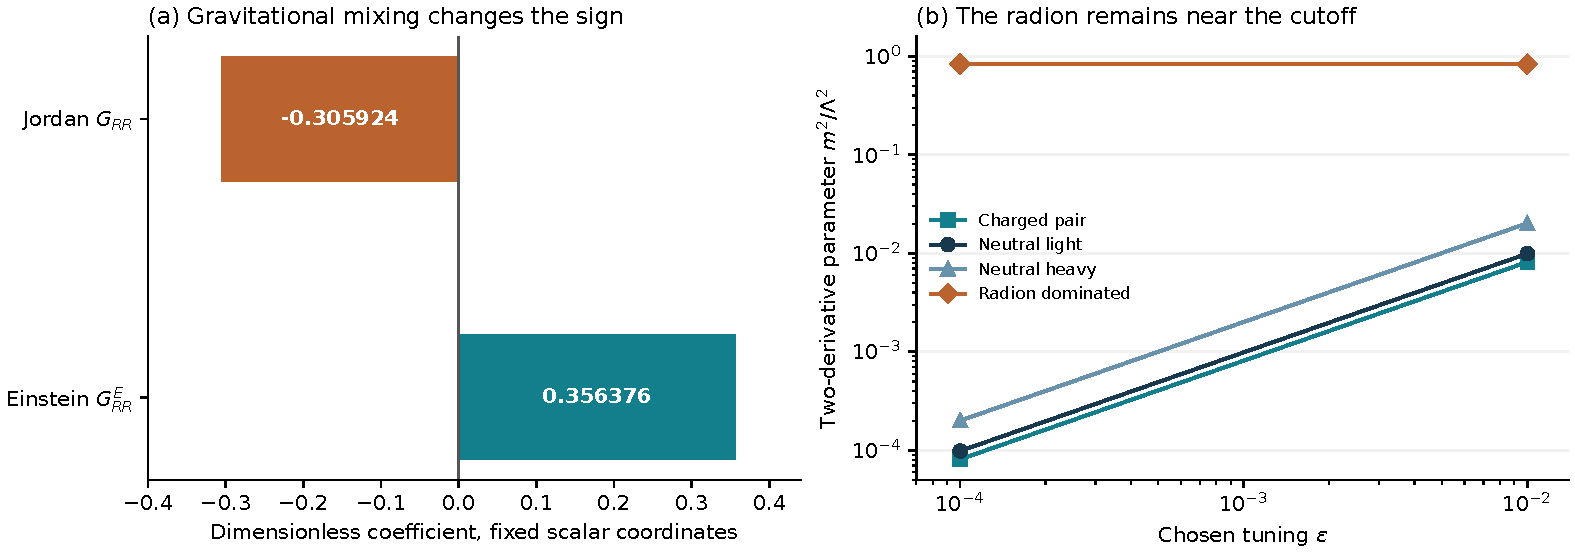
\includegraphics[width=\linewidth]{images/kinetics_and_scales.pdf}
 \caption{Minus-profile diagnostics. (a) Jordan and Einstein radial entries at $\epsilon=0.01$, with all scalar coordinates fixed. Physical scalar positivity uses the full Einstein matrix. (b) Generalized squared-mass parameters of the two-derivative action. The radion remains near the spectral cutoff as the scalar tuning decreases. Lines connect the two computed fixtures; they are not an independently sampled branch.}
\end{figure}

A further check evaluates the full scalar/radius two-point kernel on a \emph{fixed flat Jordan metric}. Writing $z=p_E^2/\Lam^2$, its change from zero momentum is
\begin{multline}
 \Pi_{AB}(z)-\Pi_{AB}(0)=\frac1{8\pi^2}\sum_{a,s}w_an_s
 \operatorname{Re}\sum_{ij}\int_0^1\!\dd t\,e^{-a[tb_i^2+(1-t)b_j^2]}\\
 \times\left[z e^{-at(1-t)z}(T_A)_{ij}(T_B)_{ji}
 +(e^{-at(1-t)z}-1)(A_A)_{ij}(A_B)_{ji}\right].
 \label{eq:momentum}
\end{multline}
Its derivative at zero is \eqref{eq:GJ}. At positive Euclidean $z=0.8295963$, the neutral-amplitude submatrix of $[\Pi(z)-\Pi(0)]/z$ differs in norm from its zero-momentum value by $22.6\%$. The radial entry differs by about $1.14\%$. The large cancellation between Jordan and metric-induced terms means that neither number estimates the physical radion pole shift. The omitted momentum-dependent metric response and Lorentzian continuation are required for that calculation. The full spectral action can have very different ultraviolet behavior from a finite derivative expansion \cite{spectral}.

\clearpage
\section{Reproduction, checks, and claim boundaries}

The bundle supplies the unchanged inherited operators and inputs, the new radius and full-scalar kernels, an offline runner, generated tables/figure, complete matrices/eigenvectors, and checks with explicit tolerances. There are \textbf{109 passing targeted checks}; the count measures computational checks, not independent physical predictions.

\begin{center}
\small
\begin{tabular}{p{0.64\linewidth}r}
\toprule Check & Observed discrepancy\\\midrule
Direct exponential-quadrature vs. eigenbasis radion/scalar metric & $3.9\times10^{-15}$\\
Dense angular vs. magnetic-block charged metric & $2.2\times10^{-16}$\\
Analytic gravitational gradient vs. finite differences & $3.1\times10^{-11}$\\
External round-$S^4$ gravity extraction vs. Eq.~\eqref{eq:f} & $1.2\times10^{-9}$\\
Finite-difference Einstein potential Hessian at the flat fixture & $6.6\times10^{-9}$\\
\bottomrule
\end{tabular}
\end{center}
The last two are controlled finite-step extrapolations, not interval enclosures. The runner also checks the unbroken heat sums, the six-dimensional Einstein-Hilbert limit, cutoff 12 versus 16, preservation of the previous scalar metric and charged curvature, the neutral phase/gauge Ward identity, generalized-eigenvector residuals and normalization, and coordinate invariance. Its cutoffs apply to fermion angular sums, not to a complete bosonic mode reduction.

The following qualifications are part of the result, and are repeated in \texttt{ASSUMPTIONS.md}:
\begin{enumerate}
 \item \textbf{Conditional operator and background.} The microscopic insertion, torsion-free warped round sphere, fixed monopole connection, four copied blocks and unit Yukawas are inherited specifications. Their uniqueness, phenomenological viability, and six-dimensional ultraviolet completion are not established. The fixed cutoff $\Lam$ is not promoted to a dilaton.
 \item \textbf{Chosen extra potential.} The positive scalar-mass counterterm is externally selected and common to the profiles. Flatness fixes $c$ separately for each fixture; $c$ is held fixed in derivatives. This is not a cosmological-constant solution. The extra operators are assumed to supply no additional derivative or curvature terms. Unspecified kinetic, gravitational or nonminimal counterterms could change the answer.
 \item \textbf{Precise stability scope.} The retained nine-field Einstein kinetic matrix is positive, and the restricted two-derivative potential Hessian is nonnegative with the symmetry zeros. This establishes the corresponding local infrared quadratic tests. It does not establish stability of a complete six-dimensional vacuum, because higher scalar harmonics, nonspherical metric modes, other gauge/bosonic fluctuations and their tadpoles have not been solved or integrated out.
 \item \textbf{Heavy-mode limitation.} The radion-dominated mass parameter is near $\Lam$. Higher external derivatives, momentum-dependent metric mixing and full Lorentzian poles/residues are unresolved. A Euclidean heat trace does not by itself prove reflection positivity or a unitary ultraviolet continuation. No claim of absence of higher-derivative gravitational ghosts is made. The fixed-metric momentum diagnostic does not fill this gap.
 \item \textbf{Gauge and axion sector.} The neutral Ward identity is checked, and the predecessor's neutral gauge kinetic positivity is inherited. The full charged-vector response and complete gauge/metric fluctuation system are not supplied here. A potential-free axion with a positive independent kinetic coefficient and pure-$X$ Stueckelberg coupling is assumed; extra axion derivative mixing is not derived. One physical phase remains massless. The anomaly polynomial, two-form reduction, axion potential and Stueckelberg scale remain unspecified.
 \item \textbf{Local, numerical and classical.} No global minimality, uniqueness, vacuum lifetime or nonlinear stability is proved. The untuned runaway remains an inherited separate result. New values use float64/complex128 finite-cutoff arithmetic with convergence checks, not interval certificates or a uniform tail bound. Small profile differences carry fewer reliable digits than absolute values. These are classical spectral-action calculations, not a loop effective potential.
 \item \textbf{No empirical normalization or external review.} The calculation selects neither $\kappa$, $\Lam$, nor a physical profile, and computes no quantum matching or running. No measured coupling is fitted; the measured fine-structure constant remains unexplained. The review is an AI-assisted same-session self-audit with independent computational paths, not a separate-agent referee or external peer review.
\end{enumerate}

\section{Next calculation made precise}

The missing radion coefficient at two derivatives is now replaced by an explicit spectral formula and checked numerical matrices. The next dynamical question is the coupled metric/radion/scalar two-point operator at finite external momentum, including the graviton constraints, followed by a stated Lorentzian prescription and pole/residue analysis. Separately, higher-harmonic tadpoles and the full bosonic fluctuation spectrum are needed to decide whether the retained stationary family embeds in a genuine compactification vacuum. The light scalar tuning does not itself create a radion-to-cutoff hierarchy.

\begin{thebibliography}{9}\small
\bibitem{vacuum} Baird / ZoraASI research continuation, prepared with OpenAI Codex,
\emph{Exact scalar-radius vacuum: instability and tuned stationary branches} (22 October 2026),
\href{https://github.com/Cbaird26/mqgt-scf-continued/releases/tag/v2026.10.22-exact-coupled-vacuum}{research prerelease}, source commit \texttt{8ac07feb}.
\bibitem{exact} Baird / ZoraASI research continuation, prepared with OpenAI Codex,
\emph{Exact internal mode sums for the scalar sector and Higgs-induced neutral kinetics} (22 October 2026),
\href{https://github.com/Cbaird26/mqgt-scf-continued/releases/tag/v2026.10.22-exact-scalar-mode-sums}{research prerelease}.
\bibitem{warped} M. B. Law, I. M. Lopez and D. Santiago,
\emph{Positive mass and Dirac operators on weighted manifolds and smooth metric measure spaces},
\href{https://arxiv.org/abs/2312.15441}{arXiv:2312.15441}, Theorem 3.5, especially Eq. (3.27).
\bibitem{heat} D. V. Vassilevich, \emph{Heat kernel expansion: user's manual},
Phys. Rept. \textbf{388} (2003) 279--360,
\href{https://arxiv.org/abs/hep-th/0306138}{arXiv:hep-th/0306138}, Sections 3.3 and 4.1.
\bibitem{kaiser} D. I. Kaiser, \emph{Conformal transformations with multiple scalar fields},
Phys. Rev. D \textbf{81} (2010) 084044,
\href{https://arxiv.org/abs/1003.1159}{arXiv:1003.1159}, Eqs. (29)--(32).
\bibitem{spectral} B. Iochum, C. Levy and D. Vassilevich,
\emph{Spectral action beyond the weak-field approximation},
Commun. Math. Phys. \textbf{316} (2012) 595--613,
\href{https://arxiv.org/abs/1108.3749}{arXiv:1108.3749}.
\end{thebibliography}

\end{document}
